
\section{Physics / Thermodynamics}


\subsection{Work Done in a Cyclic Process}


A thermodynamic system undergoes a cyclic process $ABC$ as shown in the diagram. The work done by the system per cycle is \underline{\hspace{2cm}}.

\begin{center}

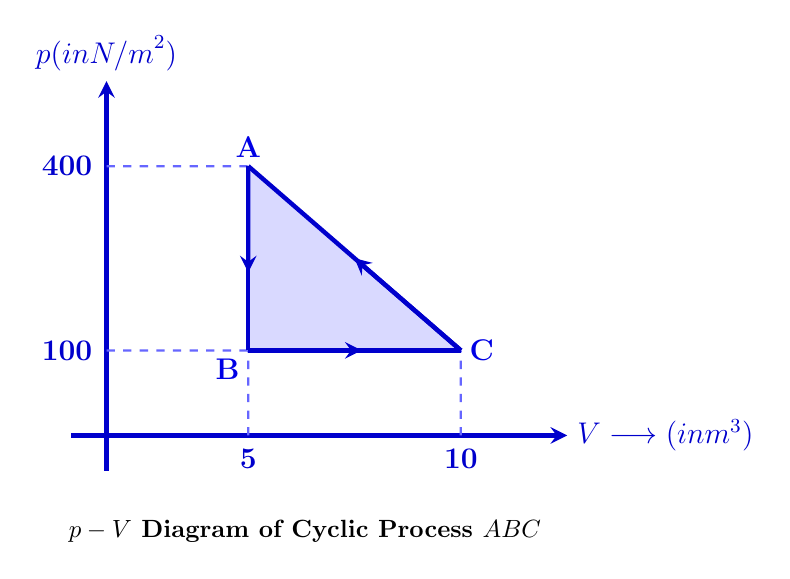
\begin{tikzpicture}[scale=0.9, every node/.style={scale=0.9}]
    % P-V Diagram for Cyclic Process ABC
    \begin{scope}[shift={(0,0)}]
        % Axes
        \draw[ultra thick, ->, >=stealth, blue!80!black] (-0.5, 0) -- (6.5, 0) node[right, font=\large\bfseries] {$V \longrightarrow (\text{in m}^3)$};
        \draw[ultra thick, ->, >=stealth, blue!80!black] (0, -0.5) -- (0, 5.0) node[above, font=\large\bfseries] {$p (\text{in N/m}^2)$};

        % Coordinates:
        % B = (2.0, 1.2), A = (2.0, 3.8), C = (5.0, 1.2)
        \coordinate (B) at (2.0, 1.2);
        \coordinate (A) at (2.0, 3.8);
        \coordinate (C) at (5.0, 1.2);

        % Dashed lines to axes
        \draw[dashed, thick, blue!60] (0, 3.8) node[left=2pt, font=\large\bfseries, blue!80!black] {400} -- (A);
        \draw[dashed, thick, blue!60] (0, 1.2) node[left=2pt, font=\large\bfseries, blue!80!black] {100} -- (B);

        \draw[dashed, thick, blue!60] (2.0, 0) node[below=2pt, font=\large\bfseries, blue!80!black] {5} -- (B);
        \draw[dashed, thick, blue!60] (5.0, 0) node[below=2pt, font=\large\bfseries, blue!80!black] {10} -- (C);

        % Shaded area of cyclic process
        \fill[blue!15] (A) -- (B) -- (C) -- cycle;

        % Cyclic paths with direction arrows (Clockwise ABC)
        % A -> B
        \draw[ultra thick, blue!80!black] (A) -- (B);
        \draw[ultra thick, ->, >=stealth, blue!80!black] (A) -- (2.0, 2.3);

        % B -> C
        \draw[ultra thick, blue!80!black] (B) -- (C);
        \draw[ultra thick, ->, >=stealth, blue!80!black] (B) -- (3.6, 1.2);

        % C -> A
        \draw[ultra thick, blue!80!black] (C) -- (A);
        \draw[ultra thick, ->, >=stealth, blue!80!black] (C) -- (3.5, 2.5);

        % Point Labels
        \node[above, font=\large\bfseries, blue!90!black] at (A) {A};
        \node[below left, font=\large\bfseries, blue!90!black] at (B) {B};
        \node[right, font=\large\bfseries, blue!90!black] at (C) {C};

        \node[below=25pt, font=\bfseries] at (2.8,-0.2) {$p-V$ Diagram of Cyclic Process $ABC$};
    \end{scope}
\end{tikzpicture}  
\end{center}


\begin{choices}
    \correctchoice $750\text{ J}$
    \choice $-1250\text{ J}$
    \choice $-750\text{ J}$
    \choice $1250\text{ J}$
\end{choices}

\begin{solution}
\subsection*{Understand Work Done in a Cyclic Process}
The net work done by a thermodynamic system in a closed cyclic process on a $p-V$ diagram is given by the area enclosed by the cycle:

\begin{itemize}
    \item **Clockwise Cycle:** Work done is **positive** ($W > 0$).
    \item **Counter-Clockwise Cycle:** Work done is **negative** ($W < 0$).
\end{itemize}

\begin{empheq}[box={\mymath[colback=col3!30,drop lifted shadow, rounded corners]}]{equation}\tag{Cyclic Work Formula}
W_{\text{net}} = +\text{Area of } \Delta ABC \quad (\text{since direction is clockwise } A \to B \to C \to A)
\end{empheq}

\subsection*{Step 1: Calculate Dimensions of Triangle $\Delta ABC$}
From the given $p-V$ plot:
\begin{itemize}
    \item **Base ($BC$):** 
    $$\text{Base} = V_C - V_B = 10\text{ m}^3 - 5\text{ m}^3 = 5\text{ m}^3$$

    \item **Height ($AB$):** 
    $$\text{Height} = p_A - p_B = 400\text{ N/m}^2 - 100\text{ N/m}^2 = 300\text{ N/m}^2$$
\end{itemize}

\subsection*{Step 2: Calculate Area of Triangle $\Delta ABC$}
$$W = \frac{1}{2} \times \text{Base} \times \text{Height}$$

$$W = \frac{1}{2} \times (5\text{ m}^3) \times (300\text{ N/m}^2) = 750\text{ J}$$

Since the cycle goes clockwise ($A \to B \to C \to A$), the net work done by the system per cycle is positive:

$$W = +750\text{ J}$$

Correct Answer: A ($750\text{ J}$)
\end{solution}

\clearpage



\section{Physics / Electrostatics \& Capacitance}


\subsection{Equivalent Capacitance and Voltage Distribution}


In the circuit shown in the figure, the potential difference across the $4\,\mu\text{F}$ capacitor is \underline{\hspace{2cm}}.

\begin{center}

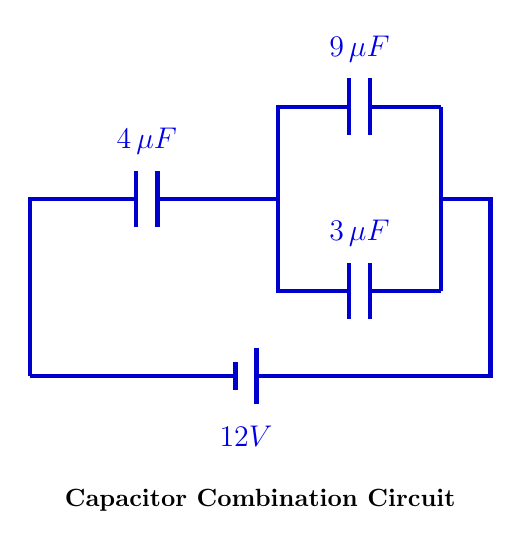
\begin{tikzpicture}[scale=0.9, every node/.style={scale=0.9}]
    % Circuit Schematic
    \begin{scope}[shift={(0,0)}]
        % Coordinates
        % Battery at bottom
        % 4 uF on main series branch
        % 9 uF and 3 uF in parallel
        
        % Main loop wire
        \draw[ultra thick, blue!80!black] (0,0) -- (0,2.5) -- (1.5,2.5);
        
        % 4 uF Capacitor
        \draw[ultra thick, blue!80!black] (1.5,2.1) -- (1.5,2.9);
        \draw[ultra thick, blue!80!black] (1.8,2.1) -- (1.8,2.9);
        \node[above=3pt, font=\large\bfseries, blue!90!black] at (1.65,2.9) {$4\,\mu\text{F}$};
        
        \draw[ultra thick, blue!80!black] (1.8,2.5) -- (3.5,2.5);
        
        % Parallel junction left vertical wire
        \draw[ultra thick, blue!80!black] (3.5,2.5) -- (3.5,3.8) -- (4.5,3.8);
        \draw[ultra thick, blue!80!black] (3.5,2.5) -- (3.5,1.2) -- (4.5,1.2);
        
        % 9 uF Capacitor (top parallel branch)
        \draw[ultra thick, blue!80!black] (4.5,3.4) -- (4.5,4.2);
        \draw[ultra thick, blue!80!black] (4.8,3.4) -- (4.8,4.2);
        \node[above=3pt, font=\large\bfseries, blue!90!black] at (4.65,4.2) {$9\,\mu\text{F}$};
        \draw[ultra thick, blue!80!black] (4.8,3.8) -- (5.8,3.8);
        
        % 3 uF Capacitor (bottom parallel branch)
        \draw[ultra thick, blue!80!black] (4.5,0.8) -- (4.5,1.6);
        \draw[ultra thick, blue!80!black] (4.8,0.8) -- (4.8,1.6);
        \node[above=3pt, font=\large\bfseries, blue!90!black] at (4.65,1.6) {$3\,\mu\text{F}$};
        \draw[ultra thick, blue!80!black] (4.8,1.2) -- (5.8,1.2);
        
        % Parallel junction right vertical wire
        \draw[ultra thick, blue!80!black] (5.8,3.8) -- (5.8,1.2);
        \draw[ultra thick, blue!80!black] (5.8,2.5) -- (6.5,2.5) -- (6.5,0) -- (3.5,0);
        
        % Battery at bottom branch
        \draw[ultra thick, blue!80!black] (3.5,0) -- (3.2,0);
        \draw[ultra thick, blue!80!black] (3.2,0.4) -- (3.2,-0.4); % Long plate (+)
        \draw[ultra thick, blue!80!black] (2.9,0.2) -- (2.9,-0.2); % Short plate (-)
        \draw[ultra thick, blue!80!black] (2.9,0) -- (0,0);
        
        \node[below=5pt, font=\large\bfseries, blue!90!black] at (3.05,-0.4) {$12\text{ V}$};

        \node[below=25pt, font=\bfseries] at (3.25,-0.6) {Capacitor Combination Circuit};
    \end{scope}
\end{tikzpicture}  
\end{center}


\begin{choices}
    \choice $3\text{ V}$
    \choice $4\text{ V}$
    \correctchoice $9\text{ V}$
    \choice $12\text{ V}$
\end{choices}

\begin{solution}
\subsection*{Understand Circuit Analysis for Capacitors}
To find the potential difference across the $4\,\mu\text{F}$ capacitor, we analyze the circuit in two steps:
1. Combine the parallel capacitors into an equivalent capacitance $C_p$.
2. Treat the resulting circuit as a simple series combination across the $12\text{ V}$ voltage source.

\begin{empheq}[box={\mymath[colback=col3!30,drop lifted shadow, rounded corners]}]{equation}\tag{Voltage Divider for Series Capacitors}
V_1 = V_{\text{total}} \cdot \frac{C_{\text{eq}}}{C_1} = V_{\text{total}} \cdot \frac{C_2}{C_1 + C_2}
\end{empheq}

\subsection*{Step 1: Find Equivalent Capacitance of the Parallel Combination}
The $9\,\mu\text{F}$ and $3\,\mu\text{F}$ capacitors are connected in parallel. Their combined equivalent capacitance $C_p$ is:

$$C_p = 9\,\mu\text{F} + 3\,\mu\text{F} = 12\,\mu\text{F}$$

\subsection*{Step 2: Series Combination with $4\,\mu\text{F}$ Capacitor}
Now, the circuit reduces to a series combination of two capacitors:
\begin{itemize}
    \item $C_1 = 4\,\mu\text{F}$
    \item $C_p = 12\,\mu\text{F}$
\end{itemize}

The net equivalent capacitance $C_{\text{eq}}$ of the entire circuit is given by:

$$\frac{1}{C_{\text{eq}}} = \frac{1}{C_1} + \frac{1}{C_p} = \frac{1}{4} + \frac{1}{12} = \frac{3 + 1}{12} = \frac{4}{12} = \frac{1}{3}$$

$$C_{\text{eq}} = 3\,\mu\text{F}$$

\subsection*{Step 3: Calculate Potential Difference across $4\,\mu\text{F}$ Capacitor}
The total charge $Q$ supplied by the $12\text{ V}$ battery is:

$$Q = C_{\text{eq}} \cdot V_{\text{total}} = (3\,\mu\text{F}) \times (12\text{ V}) = 36\,\mu\text{C}$$

Since $C_1 = 4\,\mu\text{F}$ is connected in series with the battery, the full charge $Q = 36\,\mu\text{C}$ flows through it. Therefore, the potential difference $V_1$ across the $4\,\mu\text{F}$ capacitor is:

$$V_1 = \frac{Q}{C_1} = \frac{36\,\mu\text{C}}{4\,\mu\text{F}} = 9\text{ V}$$

Alternatively, using the voltage divider rule:

$$V_1 = 12\text{ V} \times \frac{C_p}{C_1 + C_p} = 12 \times \frac{12}{4 + 12} = 12 \times \frac{12}{16} = 9\text{ V}$$

Thus, the potential difference across the $4\,\mu\text{F}$ capacitor is **$9\text{ V}$**.

Correct Answer: C ($9\text{ V}$)
\end{solution}

\clearpage

\section{Physics / Electrostatics \& Capacitance}


\subsection{Parallel Plate Capacitor with Dielectric Slab}


If a slab of insulating material $4 \times 10^{-3}\text{ m}$ thick is introduced between the plates of a parallel plate capacitor, the separation between the plates has to be increased by $3.5 \times 10^{-3}\text{ m}$ to restore the capacity to its original value. The dielectric constant of the material will be \underline{\hspace{2cm}}.

\begin{center}

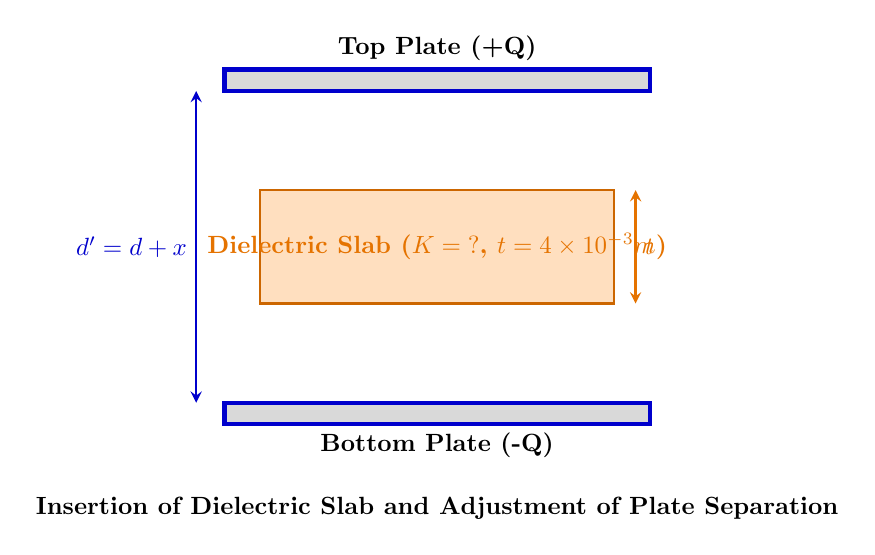
\begin{tikzpicture}[scale=0.9, every node/.style={scale=0.9}]
    % Parallel Plate Capacitor Schematic with Dielectric Slab
    \begin{scope}[shift={(0,0)}]
        % Top Plate
        \draw[ultra thick, fill=gray!30, draw=blue!80!black] (-3, 2.2) rectangle (3, 2.5);
        \node[above, font=\bfseries] at (0, 2.5) {Top Plate (+Q)};

        % Bottom Plate
        \draw[ultra thick, fill=gray!30, draw=blue!80!black] (-3, -2.5) rectangle (3, -2.2);
        \node[below, font=\bfseries] at (0, -2.5) {Bottom Plate (-Q)};

        % Dielectric Slab
        \draw[thick, fill=orange!25, draw=orange!80!black] (-2.5, -0.8) rectangle (2.5, 0.8);
        \node[font=\bfseries, orange!90!black] at (0, 0) {Dielectric Slab ($K = \text{?}$, $t = 4 \times 10^{-3}\text{ m}$)};

        % Plate separation dimension d + x
        \draw[thick, <->, >=stealth, blue!80!black] (-3.4, -2.2) -- (-3.4, 2.2) node[midway, left, font=\bfseries] {$d' = d + x$};

        % Slab thickness dimension t
        \draw[thick, <->, >=stealth, orange!90!black] (2.8, -0.8) -- (2.8, 0.8) node[midway, right, font=\bfseries] {$t$};

        \node[below=20pt, font=\bfseries] at (0,-2.7) {Insertion of Dielectric Slab and Adjustment of Plate Separation};
    \end{scope}
\end{tikzpicture}  
\end{center}


\begin{choices}
    \choice $6$
    \correctchoice $8$
    \choice $10$
    \choice $12$
\end{choices}

\begin{solution}
\subsection*{Understand Capacitance with Partial Dielectric Slab}
For a parallel plate capacitor with plate area $A$ and initial plate separation $d$, the initial capacitance in air/vacuum is:

$$C_0 = \frac{\varepsilon_0 A}{d}$$

When a dielectric slab of thickness $t$ and dielectric constant $K$ is introduced, the capacitance becomes:

$$C = \frac{\varepsilon_0 A}{d - t + \frac{t}{K}} = \frac{\varepsilon_0 A}{d - t\left(1 - \frac{1}{K}\right)}$$

\begin{empheq}[box={\mymath[colback=col3!30,drop lifted shadow, rounded corners]}]{equation}\tag{Apparent Shift Equation}
x = t\left(1 - \frac{1}{K}\right)
\end{empheq}

\subsection*{Step 1: Relate Distance Adjustment to Slab Parameters}
To restore the capacitance to its original value $C_0$, the separation between the plates is increased by a distance $x$ ($d' = d + x$):

$$C' = \frac{\varepsilon_0 A}{(d + x) - t + \frac{t}{K}} = C_0 = \frac{\varepsilon_0 A}{d}$$

Equating the denominators:

$$(d + x) - t + \frac{t}{K} = d$$

$$x = t - \frac{t}{K} = t\left(1 - \frac{1}{K}\right)$$

\subsection*{Step 2: Calculate Dielectric Constant ($K$)}
Given values:
\begin{itemize}
    \item Thickness of dielectric slab, $t = 4 \times 10^{-3}\text{ m}$
    \item Increase in plate separation, $x = 3.5 \times 10^{-3}\text{ m}$
\end{itemize}

Substitute $t$ and $x$ into the equation:

$$3.5 \times 10^{-3} = 4 \times 10^{-3} \left(1 - \frac{1}{K}\right)$$

$$\frac{3.5}{4} = 1 - \frac{1}{K}$$

$$0.875 = 1 - \frac{1}{K}$$

$$\frac{1}{K} = 1 - 0.875 = 0.125 = \frac{1}{8}$$

$$K = 8$$

Thus, the dielectric constant of the material is **$8$**.

Correct Answer: B ($8$)
\end{solution}

\clearpage

\section{Physics / Electrostatics \& Capacitance}


\subsection{Grouping of Identical Capacitors for Desired Voltage and Capacitance}


An electrician requires a capacitance of $6\,\mu\text{F}$ in a circuit across a potential difference of $1.5\text{ kV}$. A large number of $2\,\mu\text{F}$ capacitors which can withstand a potential difference of not more than $500\text{ V}$ are available. The minimum number of capacitors required for the purpose is \underline{\hspace{2cm}}.

\begin{center}

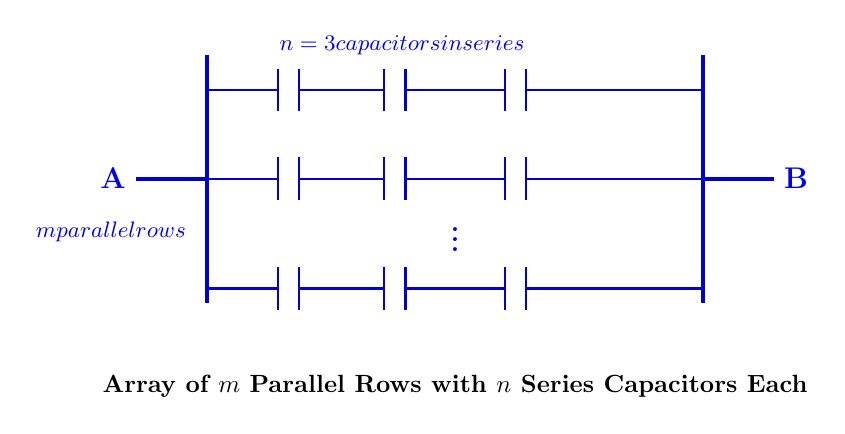
\begin{tikzpicture}[scale=0.9, every node/.style={scale=0.9}]
    % Capacitor Array Schematic (m rows of n capacitors in series)
    \begin{scope}[shift={(0,0)}]
        % Total Voltage Bus Bars
        \draw[ultra thick, blue!80!black] (-1,0) -- (-1,3.5);
        \draw[ultra thick, blue!80!black] (6,0) -- (6,3.5);
        \draw[ultra thick, blue!80!black] (-1,1.75) -- (-2,1.75) node[left, font=\large\bfseries, blue!90!black] {A};
        \draw[ultra thick, blue!80!black] (6,1.75) -- (7,1.75) node[right, font=\large\bfseries, blue!90!black] {B};

        % Row 1
        \draw[thick, blue!80!black] (-1,3) -- (0,3);
        \draw[thick, blue!80!black] (0,2.7) -- (0,3.3); \draw[thick, blue!80!black] (0.3,2.7) -- (0.3,3.3);
        \draw[thick, blue!80!black] (0.3,3) -- (1.5,3);
        \draw[thick, blue!80!black] (1.5,2.7) -- (1.5,3.3); \draw[thick, blue!80!black] (1.8,2.7) -- (1.8,3.3);
        \draw[thick, blue!80!black] (1.8,3) -- (3.2,3);
        \draw[thick, blue!80!black] (3.2,2.7) -- (3.2,3.3); \draw[thick, blue!80!black] (3.5,2.7) -- (3.5,3.3);
        \draw[thick, blue!80!black] (3.5,3) -- (6,3);
        \node[above=2pt, font=\small\bfseries, blue!90!black] at (1.75,3.3) {$n = 3 \text{ capacitors in series}$};

        % Row 2
        \draw[thick, blue!80!black] (-1,1.75) -- (0,1.75);
        \draw[thick, blue!80!black] (0,1.45) -- (0,2.05); \draw[thick, blue!80!black] (0.3,1.45) -- (0.3,2.05);
        \draw[thick, blue!80!black] (0.3,1.75) -- (1.5,1.75);
        \draw[thick, blue!80!black] (1.5,1.45) -- (1.5,2.05); \draw[thick, blue!80!black] (1.8,1.45) -- (1.8,2.05);
        \draw[thick, blue!80!black] (1.8,1.75) -- (3.2,1.75);
        \draw[thick, blue!80!black] (3.2,1.45) -- (3.2,2.05); \draw[thick, blue!80!black] (3.5,1.45) -- (3.5,2.05);
        \draw[thick, blue!80!black] (3.5,1.75) -- (6,1.75);

        % Vertical dots for m rows
        \node[font=\bfseries, blue!80!black] at (2.5,1.0) {$\vdots$};
        \node[left=5pt, font=\small\bfseries, blue!90!black] at (-1,1.0) {$m \text{ parallel rows}$};

        % Row m
        \draw[thick, blue!80!black] (-1,0.2) -- (0,0.2);
        \draw[thick, blue!80!black] (0,-0.1) -- (0,0.5); \draw[thick, blue!80!black] (0.3,-0.1) -- (0.3,0.5);
        \draw[thick, blue!80!black] (0.3,0.2) -- (1.5,0.2);
        \draw[thick, blue!80!black] (1.5,-0.1) -- (1.5,0.5); \draw[thick, blue!80!black] (1.8,-0.1) -- (1.8,0.5);
        \draw[thick, blue!80!black] (1.8,0.2) -- (3.2,0.2);
        \draw[thick, blue!80!black] (3.2,-0.1) -- (3.2,0.5); \draw[thick, blue!80!black] (3.5,-0.1) -- (3.5,0.5);
        \draw[thick, blue!80!black] (3.5,0.2) -- (6,0.2);

        \node[below=20pt, font=\bfseries] at (2.5,-0.2) {Array of $m$ Parallel Rows with $n$ Series Capacitors Each};
    \end{scope}
\end{tikzpicture}  
\end{center}


\begin{choices}
    \choice $3$
    \choice $9$
    \choice $6$
    \correctchoice $27$
\end{choices}

\begin{solution}
\subsection*{Understand Capacitor Network Formulation}
To achieve a required total capacitance $C_{\text{eq}}$ across a high potential difference $V_{\text{total}}$, we connect $n$ identical capacitors in series within each branch, and place $m$ such identical branches in parallel.

\begin{itemize}
    \item Individual capacitance = $C = 2\,\mu\text{F}$
    \item Maximum safe voltage per capacitor = $V_0 = 500\text{ V}$
    \item Required net potential difference = $V_{\text{total}} = 1.5\text{ kV} = 1500\text{ V}$
    \item Required net equivalent capacitance = $C_{\text{eq}} = 6\,\mu\text{F}$
\end{itemize}

\begin{empheq}[box={\mymath[colback=col3!30,drop lifted shadow, rounded corners]}]{equation}\tag{Capacitor Grouping Formulas}
n = \frac{V_{\text{total}}}{V_0}, \quad C_{\text{branch}} = \frac{C}{n}, \quad C_{\text{eq}} = m \cdot C_{\text{branch}} = \frac{m \cdot C}{n}
\end{empheq}

\subsection*{Step 1: Determine the Number of Capacitors in Series per Branch ($n$)}
Since each capacitor can safely withstand a maximum voltage of $V_0 = 500\text{ V}$, the total voltage $V_{\text{total}} = 1500\text{ V}$ must be divided equally across $n$ capacitors connected in series:

$$n = \frac{V_{\text{total}}}{V_0} = \frac{1500\text{ V}}{500\text{ V}} = 3\text{ capacitors per branch}$$

\subsection*{Step 2: Calculate Equivalent Capacitance of One Series Branch ($C_{\text{branch}}$)}
For $n = 3$ identical capacitors of $C = 2\,\mu\text{F}$ connected in series:

$$C_{\text{branch}} = \frac{C}{n} = \frac{2\,\mu\text{F}}{3}$$

\subsection*{Step 3: Determine the Number of Parallel Branches ($m$)}
To obtain the desired total equivalent capacitance $C_{\text{eq}} = 6\,\mu\text{F}$, we connect $m$ such identical branches in parallel:

$$C_{\text{eq}} = m \cdot C_{\text{branch}}$$

$$6\,\mu\text{F} = m \cdot \left(\frac{2\,\mu\text{F}}{3}\right)$$

$$m = \frac{6 \times 3}{2} = 9\text{ branches}$$

\subsection*{Step 4: Calculate Minimum Total Number of Capacitors ($N$)}
The total number of capacitors $N$ required in the network is:

$$N = m \times n = 9 \times 3 = 27$$

Thus, the minimum number of capacitors required is **$27$**.

Correct Answer: D ($27$)
\end{solution}

\clearpage

\section{Physics / Electrostatics \& Capacitance}


\subsection{Charge vs Potential Difference ($Q-V$) Graph Analysis}


In figure, charge on the capacitor is plotted against potential difference across the capacitor. The capacitance and energy stored in the capacitor are respectively \underline{\hspace{2cm}}.

\begin{center}

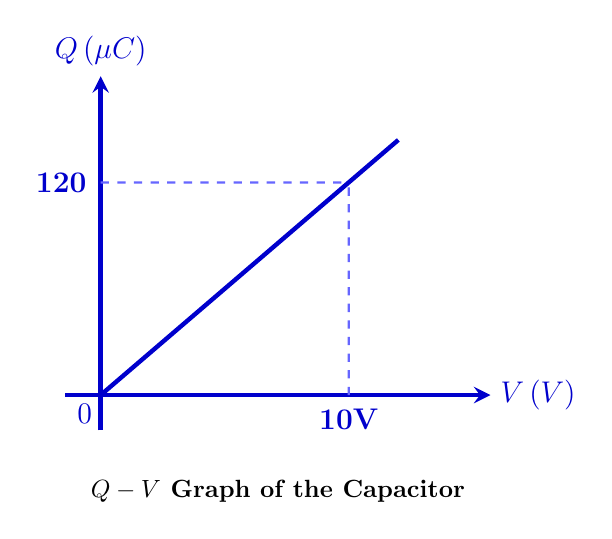
\begin{tikzpicture}[scale=0.9, every node/.style={scale=0.9}]
    % Q-V Graph
    \begin{scope}[shift={(0,0)}]
        % Axes
        \draw[ultra thick, ->, >=stealth, blue!80!black] (-0.5, 0) -- (5.5, 0) node[right, font=\large\bfseries] {$V\,\text{(V)}$};
        \draw[ultra thick, ->, >=stealth, blue!80!black] (0, -0.5) -- (0, 4.5) node[above, font=\large\bfseries] {$Q\,(\mu\text{C})$};

        % Origin
        \node[below left, font=\large\bfseries, blue!80!black] at (0,0) {$0$};

        % Point coordinates: V = 10 V, Q = 120 uC
        \coordinate (P) at (3.5, 3.0);

        % Dashed lines to axes
        \draw[dashed, thick, blue!60] (0, 3.0) node[left=2pt, font=\large\bfseries, blue!80!black] {120} -- (P);
        \draw[dashed, thick, blue!60] (3.5, 0) node[below=2pt, font=\large\bfseries, blue!80!black] {10V} -- (P);

        % Straight line Q = C * V passing through origin
        \draw[ultra thick, blue!80!black] (0,0) -- (4.2, 3.6);

        \node[below=25pt, font=\bfseries] at (2.5,-0.2) {$Q-V$ Graph of the Capacitor};
    \end{scope}
\end{tikzpicture}  
\end{center}


\begin{choices}
    \choice $12\,\mu\text{F},\,1200\,\mu\text{J}$
    \correctchoice $12\,\mu\text{F},\,600\,\mu\text{J}$
    \choice $24\,\mu\text{F},\,600\,\mu\text{J}$
    \choice $24\,\mu\text{F},\,1200\,\mu\text{J}$
\end{choices}

\begin{solution}
\subsection*{Understand Capacitance and Stored Energy Relations}
From the $Q-V$ plot, for a potential difference of $V = 10\text{ V}$, the charge accumulated on the capacitor is $Q = 120\,\mu\text{C}$.

\begin{empheq}[box={\mymath[colback=col3!30,drop lifted shadow, rounded corners]}]{equation}\tag{Capacitor Fundamental Relations}
C = \frac{Q}{V}, \quad U = \frac{1}{2} Q V = \text{Area under } Q-V \text{ graph}
\end{empheq}

\subsection*{Step 1: Calculate Capacitance ($C$)}
$$C = \frac{Q}{V} = \frac{120\,\mu\text{C}}{10\text{ V}} = 12\,\mu\text{F}$$

\subsection*{Step 2: Calculate Stored Energy ($U$)}
Using the formula for energy stored in a capacitor:

$$U = \frac{1}{2} Q V = \frac{1}{2} \times (120\,\mu\text{C}) \times (10\text{ V})$$

$$U = 60 \times 10 = 600\,\mu\text{J}$$

Thus, the capacitance is **$12\,\mu\text{F}$** and the energy stored is **$600\,\mu\text{J}$**.

Correct Answer: B ($12\,\mu\text{F},\,600\,\mu\text{J}$)
\end{solution}

\clearpage

\section{Physics / Electrostatics \& Capacitance}


\subsection{Combination of Capacitors}


The difference between equivalent capacitances of two identical capacitors connected in parallel to that in series is $6\,\mu\text{F}$. The value of capacitance of each capacitor is \underline{\hspace{2cm}}.

\begin{center}

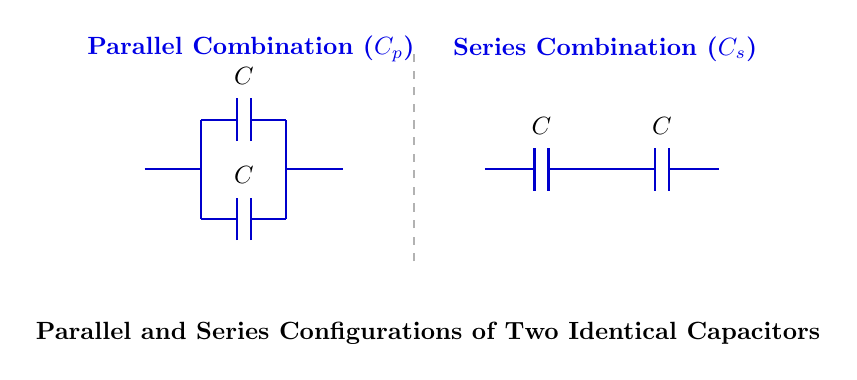
\begin{tikzpicture}[scale=0.9, every node/.style={scale=0.9}]
    % Combination Schematic (Parallel vs Series)
    \begin{scope}[shift={(0,0)}]
        % Parallel Combination (Left side)
        \node[font=\bfseries, blue!90!black] at (1.5, 3.2) {Parallel Combination ($C_p$)};
        
        \draw[thick, blue!80!black] (0, 1.5) -- (0.8, 1.5);
        \draw[thick, blue!80!black] (0.8, 0.8) -- (0.8, 2.2);
        
        % Top capacitor (Parallel)
        \draw[thick, blue!80!black] (0.8, 2.2) -- (1.3, 2.2);
        \draw[thick, blue!80!black] (1.3, 1.9) -- (1.3, 2.5);
        \draw[thick, blue!80!black] (1.5, 1.9) -- (1.5, 2.5);
        \node[above=2pt, font=\bfseries] at (1.4, 2.5) {$C$};
        \draw[thick, blue!80!black] (1.5, 2.2) -- (2.0, 2.2);
        
        % Bottom capacitor (Parallel)
        \draw[thick, blue!80!black] (0.8, 0.8) -- (1.3, 0.8);
        \draw[thick, blue!80!black] (1.3, 0.5) -- (1.3, 1.1);
        \draw[thick, blue!80!black] (1.5, 0.5) -- (1.5, 1.1);
        \node[above=2pt, font=\bfseries] at (1.4, 1.1) {$C$};
        \draw[thick, blue!80!black] (1.5, 0.8) -- (2.0, 0.8);
        
        \draw[thick, blue!80!black] (2.0, 0.8) -- (2.0, 2.2);
        \draw[thick, blue!80!black] (2.0, 1.5) -- (2.8, 1.5);

        % Separator line
        \draw[dashed, gray!60, thick] (3.8, 0.2) -- (3.8, 3.2);

        % Series Combination (Right side)
        \node[font=\bfseries, blue!90!black] at (6.5, 3.2) {Series Combination ($C_s$)};
        
        \draw[thick, blue!80!black] (4.8, 1.5) -- (5.5, 1.5);
        \draw[thick, blue!80!black] (5.5, 1.2) -- (5.5, 1.8);
        \draw[thick, blue!80!black] (5.7, 1.2) -- (5.7, 1.8);
        \node[above=2pt, font=\bfseries] at (5.6, 1.8) {$C$};
        
        \draw[thick, blue!80!black] (5.7, 1.5) -- (7.2, 1.5);
        \draw[thick, blue!80!black] (7.2, 1.2) -- (7.2, 1.8);
        \draw[thick, blue!80!black] (7.4, 1.2) -- (7.4, 1.8);
        \node[above=2pt, font=\bfseries] at (7.3, 1.8) {$C$};
        
        \draw[thick, blue!80!black] (7.4, 1.5) -- (8.1, 1.5);

        \node[below=15pt, font=\bfseries] at (4.0, 0) {Parallel and Series Configurations of Two Identical Capacitors};
    \end{scope}
\end{tikzpicture}  
\end{center}


\begin{choices}
    \choice $2\,\mu\text{F}$
    \choice $3\,\mu\text{F}$
    \correctchoice $4\,\mu\text{F}$
    \choice $6\,\mu\text{F}$
\end{choices}

\begin{solution}
\subsection*{Understand Equivalent Capacitance Formulas}
Let $C$ be the capacitance of each identical capacitor.

\begin{itemize}
    \item **Parallel Combination ($C_p$):** 
    $$C_p = C + C = 2C$$

    \item **Series Combination ($C_s$):** 
    $$C_s = \frac{C \cdot C}{C + C} = \frac{C}{2}$$
\end{itemize}

\begin{empheq}[box={\mymath[colback=col3!30,drop lifted shadow, rounded corners]}]{equation}\tag{Difference in Capacitances}
C_p - C_s = 2C - \frac{C}{2} = \frac{3}{2}C
\end{empheq}

\subsection*{Step 1: Calculate Capacitance $C$}
Given that the difference between the equivalent capacitances is $6\,\mu\text{F}$:

$$C_p - C_s = 6\,\mu\text{F}$$

$$\frac{3}{2}C = 6\,\mu\text{F}$$

$$C = 6 \times \frac{2}{3} = 4\,\mu\text{F}$$

Thus, the capacitance of each capacitor is **$4\,\mu\text{F}$**.

Correct Answer: C ($4\,\mu\text{F}$)
\end{solution}

\clearpage

\section{Physics / Electrostatics \& Capacitance}


\subsection{Equivalent Capacitance of Network}


The equivalent capacitance between A and B is \underline{\hspace{2cm}}.

\begin{center}

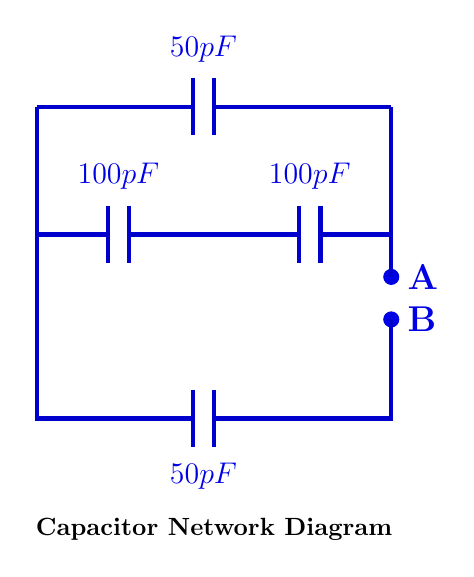
\begin{tikzpicture}[scale=0.9, every node/.style={scale=0.9}]
    % Circuit Network Diagram
    \begin{scope}[shift={(0,0)}]
        % Main outer loop coordinates
        % Top branch with 50 pF
        % Middle branch with two 100 pF capacitors
        % Bottom branch with 50 pF
        % Terminals A and B on the right side
        
        % Left Vertical Bus
        \draw[ultra thick, blue!80!black] (-2.5, 0) -- (-2.5, 3.6);
        
        % Top Branch with 50 pF
        \draw[ultra thick, blue!80!black] (-2.5, 3.6) -- (-0.3, 3.6);
        \draw[ultra thick, blue!80!black] (-0.3, 3.2) -- (-0.3, 4.0);
        \draw[ultra thick, blue!80!black] (0.0, 3.2) -- (0.0, 4.0);
        \node[above=3pt, font=\large\bfseries, blue!90!black] at (-0.15, 4.0) {$50\text{ pF}$};
        \draw[ultra thick, blue!80!black] (0.0, 3.6) -- (2.5, 3.6);
        
        % Right Vertical Bus (Top half down to A)
        \draw[ultra thick, blue!80!black] (2.5, 3.6) -- (2.5, 1.8);
        
        % Middle Branch with two 100 pF capacitors
        \draw[ultra thick, blue!80!black] (-2.5, 1.8) -- (-1.5, 1.8);
        
        % First 100 pF capacitor
        \draw[ultra thick, blue!80!black] (-1.5, 1.4) -- (-1.5, 2.2);
        \draw[ultra thick, blue!80!black] (-1.2, 1.4) -- (-1.2, 2.2);
        \node[above=3pt, font=\large\bfseries, blue!90!black] at (-1.35, 2.2) {$100\text{ pF}$};
        
        \draw[ultra thick, blue!80!black] (-1.2, 1.8) -- (1.2, 1.8);
        
        % Second 100 pF capacitor
        \draw[ultra thick, blue!80!black] (1.2, 1.4) -- (1.2, 2.2);
        \draw[ultra thick, blue!80!black] (1.5, 1.4) -- (1.5, 2.2);
        \node[above=3pt, font=\large\bfseries, blue!90!black] at (1.35, 2.2) {$100\text{ pF}$};
        
        \draw[ultra thick, blue!80!black] (1.5, 1.8) -- (2.5, 1.8);
        
        % Terminal A
        \filldraw[blue!90!black] (2.5, 1.2) circle (3pt);
        \node[right=3pt, font=\Large\bfseries, blue!90!black] at (2.5, 1.2) {A};
        \draw[ultra thick, blue!80!black] (2.5, 1.8) -- (2.5, 1.2);

        % Terminal B and Bottom Loop
        \filldraw[blue!90!black] (2.5, 0.6) circle (3pt);
        \node[right=3pt, font=\Large\bfseries, blue!90!black] at (2.5, 0.6) {B};
        \draw[ultra thick, blue!80!black] (2.5, 0.6) -- (2.5, -0.8) -- (0.0, -0.8);

        % Bottom Branch with 50 pF
        \draw[ultra thick, blue!80!black] (0.0, -1.2) -- (0.0, -0.4);
        \draw[ultra thick, blue!80!black] (-0.3, -1.2) -- (-0.3, -0.4);
        \node[below=3pt, font=\large\bfseries, blue!90!black] at (-0.15, -1.2) {$50\text{ pF}$};
        
        \draw[ultra thick, blue!80!black] (-0.3, -0.8) -- (-2.5, -0.8) -- (-2.5, 0);

        \node[below=25pt, font=\bfseries] at (0,-1.2) {Capacitor Network Diagram};
    \end{scope}
\end{tikzpicture}  
\end{center}


\begin{choices}
    \choice $50\text{ pF}$
    \correctchoice $\frac{100}{3}\text{ pF}$
    \choice $150\text{ pF}$
    \choice $300\text{ pF}$
\end{choices}

\begin{solution}
\subsection*{Understand Circuit Simplification Step-by-Step}
We analyze the network by identifying series and parallel combinations between terminals $\text{A}$ and $\text{B}$:

\begin{itemize}
    \item Let $C_1 = 50\text{ pF}$ (top capacitor)
    \item Let $C_2 = 100\text{ pF}$ and $C_3 = 100\text{ pF}$ (middle branch capacitors)
    \item Let $C_4 = 50\text{ pF}$ (bottom capacitor connected to terminal B)
\end{itemize}

\begin{empheq}[box={\mymath[colback=col3!30,drop lifted shadow, rounded corners]}]{equation}\tag{Equivalent Capacitance Formula}
C_{\text{AB}} = \frac{C_{\text{upper}} \times C_4}{C_{\text{upper}} + C_4}
\end{empheq}

\subsection*{Step 1: Simplify Middle Branch Series Combination ($C_{23}$)}
The two $100\text{ pF}$ capacitors ($C_2$ and $C_3$) are connected in series with each other:

$$C_{23} = \frac{C_2 \times C_3}{C_2 + C_3} = \frac{100 \times 100}{100 + 100} = \frac{10000}{200} = 50\text{ pF}$$

\subsection*{Step 2: Combine with Top Capacitor in Parallel ($C_{\text{upper}}$)}
This combination $C_{23} = 50\text{ pF}$ is in parallel with the top capacitor $C_1 = 50\text{ pF}$:

$$C_{\text{upper}} = C_1 + C_{23} = 50\text{ pF} + 50\text{ pF} = 100\text{ pF}$$

\subsection*{Step 3: Calculate Net Capacitance Between Terminals A and B ($C_{\text{AB}}$)}
Finally, the parallel combination $C_{\text{upper}} = 100\text{ pF}$ is in series with the bottom capacitor $C_4 = 50\text{ pF}$:

$$C_{\text{AB}} = \frac{C_{\text{upper}} \times C_4}{C_{\text{upper}} + C_4} = \frac{100 \times 50}{100 + 50} = \frac{5000}{150} = \frac{100}{3}\text{ pF}$$

Thus, the equivalent capacitance between $\text{A}$ and $\text{B}$ is **$\frac{100}{3}\text{ pF}$**.

Correct Answer: B ($\frac{100}{3}\text{ pF}$)
\end{solution}

\clearpage


    

\section{Physics / Electrostatics \& Capacitance}


\subsection{Reconnection of Capacitors}


Two capacitors of $3\,\mu\text{F}$ and $6\,\mu\text{F}$ are connected in series and a potential difference of $900\text{ V}$ is applied across the combination. They are then disconnected and reconnected in parallel. The potential difference across the combination is \underline{\hspace{2cm}}.

\begin{center}

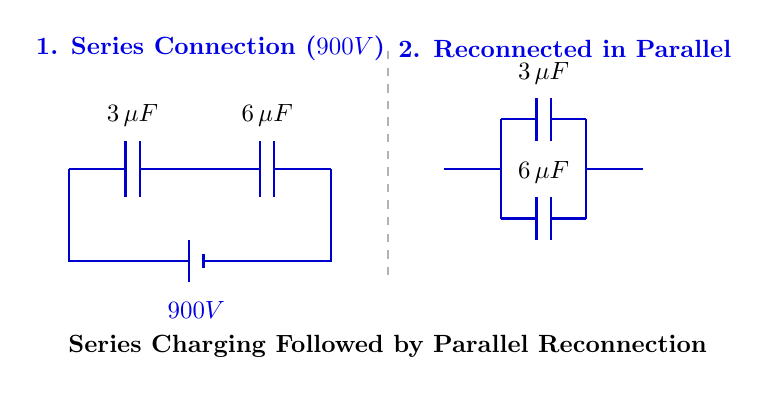
\begin{tikzpicture}[scale=0.9, every node/.style={scale=0.9}]
    % Combination Schematic (Series connection then Parallel reconnection)
    \begin{scope}[shift={(0,0)}]
        % Series Connection (Left Side)
        \node[font=\bfseries, blue!90!black] at (1.5, 3.2) {1. Series Connection ($900\text{ V}$)};
        
        \draw[thick, blue!80!black] (-0.5, 1.5) -- (0.3, 1.5);
        
        % C1 (3 uF)
        \draw[thick, blue!80!black] (0.3, 1.1) -- (0.3, 1.9);
        \draw[thick, blue!80!black] (0.5, 1.1) -- (0.5, 1.9);
        \node[above=2pt, font=\bfseries] at (0.4, 1.9) {$3\,\mu\text{F}$};
        
        \draw[thick, blue!80!black] (0.5, 1.5) -- (2.2, 1.5);
        
        % C2 (6 uF)
        \draw[thick, blue!80!black] (2.2, 1.1) -- (2.2, 1.9);
        \draw[thick, blue!80!black] (2.4, 1.1) -- (2.4, 1.9);
        \node[above=2pt, font=\bfseries] at (2.3, 1.9) {$6\,\mu\text{F}$};
        
        \draw[thick, blue!80!black] (2.4, 1.5) -- (3.2, 1.5);
        
        % Battery connection
        \draw[thick, blue!80!black] (-0.5, 1.5) -- (-0.5, 0.2) -- (1.2, 0.2);
        \draw[thick, blue!80!black] (1.2, 0.5) -- (1.2, -0.1); % Long (+)
        \draw[thick, blue!80!black] (1.4, 0.3) -- (1.4, 0.1);  % Short (-)
        \draw[thick, blue!80!black] (1.4, 0.2) -- (3.2, 0.2) -- (3.2, 1.5);
        \node[below=4pt, font=\bfseries, blue!90!black] at (1.3, -0.1) {$900\text{ V}$};

        % Separator line
        \draw[dashed, gray!60, thick] (4.0, 0.0) -- (4.0, 3.2);

        % Parallel Connection (Right Side)
        \node[font=\bfseries, blue!90!black] at (6.5, 3.2) {2. Reconnected in Parallel};
        
        \draw[thick, blue!80!black] (4.8, 1.5) -- (5.6, 1.5);
        \draw[thick, blue!80!black] (5.6, 0.8) -- (5.6, 2.2);
        
        % Top capacitor (3 uF)
        \draw[thick, blue!80!black] (5.6, 2.2) -- (6.1, 2.2);
        \draw[thick, blue!80!black] (6.1, 1.9) -- (6.1, 2.5);
        \draw[thick, blue!80!black] (6.3, 1.9) -- (6.3, 2.5);
        \node[above=2pt, font=\bfseries] at (6.2, 2.5) {$3\,\mu\text{F}$};
        \draw[thick, blue!80!black] (6.3, 2.2) -- (6.8, 2.2);
        
        % Bottom capacitor (6 uF)
        \draw[thick, blue!80!black] (5.6, 0.8) -- (6.1, 0.8);
        \draw[thick, blue!80!black] (6.1, 0.5) -- (6.1, 1.1);
        \draw[thick, blue!80!black] (6.3, 0.5) -- (6.3, 1.1);
        \node[above=2pt, font=\bfseries] at (6.2, 1.1) {$6\,\mu\text{F}$};
        \draw[thick, blue!80!black] (6.3, 0.8) -- (6.8, 0.8);
        
        \draw[thick, blue!80!black] (6.8, 0.8) -- (6.8, 2.2);
        \draw[thick, blue!80!black] (6.8, 1.5) -- (7.6, 1.5);

        \node[below=15pt, font=\bfseries] at (4.0, -0.2) {Series Charging Followed by Parallel Reconnection};
    \end{scope}
\end{tikzpicture}  
\end{center}


\begin{choices}
    \choice zero
    \choice $200\text{ V}$
    \choice $100\text{ V}$
    \correctchoice $400\text{ V}$
\end{choices}

\begin{solution}
\subsection*{Understand Reconnection Principles}
When two capacitors are charged in series and subsequently reconnected in parallel (connecting positive plates together and negative plates together), the total charge is conserved across the parallel combination.

\begin{empheq}[box={\mymath[colback=col3!30,drop lifted shadow, rounded corners]}]{equation}\tag{Common Potential Formula}
V' = \frac{Q_{\text{total}}}{C_{\text{p}}} = \frac{Q_1 + Q_2}{C_1 + C_2}
\end{empheq}

\subsection*{Step 1: Calculate Charge Received in Series Combination}
The equivalent capacitance $C_s$ of $C_1 = 3\,\mu\text{F}$ and $C_2 = 6\,\mu\text{F}$ in series is:

$$C_s = \frac{C_1 \cdot C_2}{C_1 + C_2} = \frac{3 \times 6}{3 + 6} = \frac{18}{9} = 2\,\mu\text{F}$$

The total charge supplied by the $900\text{ V}$ supply is:

$$Q = C_s \cdot V = (2\,\mu\text{F}) \times (900\text{ V}) = 1800\,\mu\text{C}$$

Since the capacitors were in series, each capacitor acquires the same charge:

$$Q_1 = 1800\,\mu\text{C}, \quad Q_2 = 1800\,\mu\text{C}$$

\subsection*{Step 2: Calculate Common Potential in Parallel Reconnection}
When reconnected in parallel, the total charge $Q_{\text{total}}$ on the parallel combination is:

$$Q_{\text{total}} = Q_1 + Q_2 = 1800\,\mu\text{C} + 1800\,\mu\text{C} = 3600\,\mu\text{C}$$

The equivalent capacitance in parallel $C_p$ is:

$$C_p = C_1 + C_2 = 3\,\mu\text{F} + 6\,\mu\text{F} = 9\,\mu\text{F}$$

Therefore, the new potential difference across the combination is:

$$V' = \frac{Q_{\text{total}}}{C_p} = \frac{3600\,\mu\text{C}}{9\,\mu\text{F}} = 400\text{ V}$$

Thus, the potential difference across the combination is **$400\text{ V}$**.

Correct Answer: D ($400\text{ V}$)
\end{solution}

\clearpage

\section{Physics / Alternating Current}


\subsection{AC Power and RMS Current Calculation}


A light bulb rated $100\text{ W}$ is connected to an AC source of $220\text{ V}, 50\text{ Hz}$. The rms current through the bulb is \underline{\hspace{2cm}}.

\begin{center}

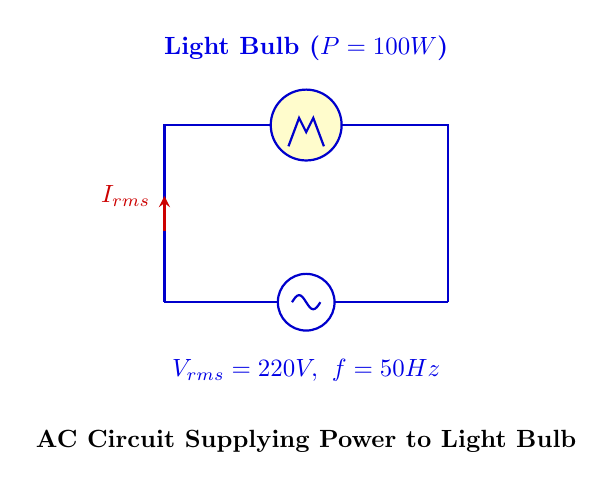
\begin{tikzpicture}[scale=0.9, every node/.style={scale=0.9}]
    % AC Circuit Diagram with Light Bulb
    \begin{scope}[shift={(0,0)}]
        % Circuit Loop Wire
        \draw[thick, blue!80!black] (-2, 0) -- (-2, 2.5) -- (2, 2.5) -- (2, 0);
        \draw[thick, blue!80!black] (-2, 0) -- (-0.4, 0);
        \draw[thick, blue!80!black] (0.4, 0) -- (2, 0);

        % AC Source at the bottom
        \draw[thick, fill=white, draw=blue!80!black] (0, 0) circle (0.4);
        \draw[thick, blue!80!black] (-0.2, 0) sin (-0.1, 0.1) cos (0, 0) sin (0.1, -0.1) cos (0.2, 0);
        \node[below=8pt, font=\bfseries, blue!90!black] at (0, -0.4) {$V_{\text{rms}} = 220\text{ V},\ f = 50\text{ Hz}$};

        % Light Bulb Schematic at the top
        \draw[thick, fill=yellow!20, draw=blue!80!black] (0, 2.5) circle (0.5);
        % Filament inside bulb
        \draw[thick, blue!80!black] (-0.25, 2.2) -- (-0.1, 2.6) -- (0, 2.4) -- (0.1, 2.6) -- (0.25, 2.2);
        \node[above=8pt, font=\bfseries, blue!90!black] at (0, 3.0) {Light Bulb ($P = 100\text{ W}$)};

        % Current Indicator Arrow
        \draw[thick, ->, >=stealth, red!80!black] (-2, 1.0) -- (-2, 1.5) node[left=2pt, font=\bfseries] {$I_{\text{rms}}$};

        \node[below=25pt, font=\bfseries] at (0, -0.8) {AC Circuit Supplying Power to Light Bulb};
    \end{scope}
\end{tikzpicture}  
\end{center}


\begin{choices}
    \correctchoice $0.454\text{ A}$
    \choice $0.545\text{ A}$
    \choice $2.20\text{ A}$
    \choice $0.22\text{ A}$
\end{choices}

\begin{solution}
\subsection*{Understand AC Power Relations}
The power dissipation $P$ in a purely resistive load (such as an incandescent light bulb) connected to an alternating voltage source is given by the product of the root-mean-square voltage ($V_{\text{rms}}$) and the root-mean-square current ($I_{\text{rms}}$).

\begin{empheq}[box={\mymath[colback=col3!30,drop lifted shadow, rounded corners]}]{equation}\tag{AC Power Formula}
P = V_{\text{rms}} \cdot I_{\text{rms}} \implies I_{\text{rms}} = \frac{P}{V_{\text{rms}}}
\end{empheq}

\subsection*{Step 1: Identify Given Parameters}
From the problem statement:
\begin{itemize}
    \item Power rating of the bulb, $P = 100\text{ W}$
    \item RMS voltage of the AC source, $V_{\text{rms}} = 220\text{ V}$
    \item Frequency of the source, $f = 50\text{ Hz}$
\end{itemize}

\subsection*{Step 2: Calculate RMS Current ($I_{\text{rms}}$)}
Substitute the values into the power equation:

$$I_{\text{rms}} = \frac{100\text{ W}}{220\text{ V}}$$

$$I_{\text{rms}} = \frac{10}{22} = \frac{5}{11}\text{ A}$$

$$I_{\text{rms}} \approx 0.4545\text{ A} \approx 0.454\text{ A}$$

Thus, the rms current passing through the light bulb is **$0.454\text{ A}$**.

Correct Answer: A ($0.454\text{ A}$)
\end{solution}

\clearpage

\section{Physics / Alternating Current}


\subsection{Phase Relationship in Purely Resistive AC Circuit}


In a circuit containing a pure resistor connected to an AC source, \underline{\hspace{3cm}}.

\begin{center}

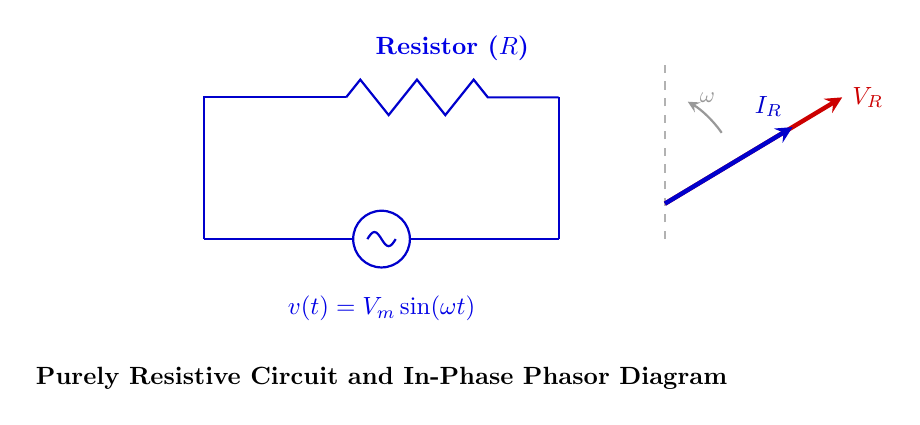
\begin{tikzpicture}[scale=0.9, every node/.style={scale=0.9}]
    % Circuit Schematic & Phasor Diagram
    \begin{scope}[shift={(0,0)}]
        % Circuit Diagram (Left)
        \draw[thick, blue!80!black] (-3.5, 0) -- (-3.5, 2) -- (-1.5, 2);
        
        % Resistor Symbol
        \draw[thick, blue!80!black] (-1.5, 2) -- (-1.3, 2.25) -- (-0.9, 1.75) -- (-0.5, 2.25) -- (-0.1, 1.75) -- (0.3, 2.25) -- (0.5, 2) -- (1.5, 2);
        \node[above=4pt, font=\bfseries, blue!90!black] at (0, 2.25) {Resistor ($R$)};

        \draw[thick, blue!80!black] (1.5, 2) -- (1.5, 0);
        \draw[thick, blue!80!black] (-3.5, 0) -- (-1.4, 0);
        \draw[thick, blue!80!black] (-0.6, 0) -- (1.5, 0);

        % AC Source Symbol
        \draw[thick, fill=white, draw=blue!80!black] (-1, 0) circle (0.4);
        \draw[thick, blue!80!black] (-1.2, 0) sin (-1.1, 0.1) cos (-1, 0) sin (-0.9, -0.1) cos (-0.8, 0);
        \node[below=8pt, font=\bfseries, blue!90!black] at (-1, -0.4) {$v(t) = V_m \sin(\omega t)$};

        % Phasor Diagram (Right)
        \draw[dashed, gray!60, thick] (3.0, 0) -- (3.0, 2.5);
        
        % Phasors collinear (in phase)
        \draw[ultra thick, ->, >=stealth, red!80!black] (3.0, 0.5) -- (5.5, 2.0) node[right, font=\bfseries] {$V_R$};
        \draw[ultra thick, ->, >=stealth, blue!80!black] (3.0, 0.5) -- (4.8, 1.58) node[above left, font=\bfseries] {$I_R$};
        
        % Angular frequency arrow
        \draw[thick, ->, >=stealth, gray!80] (3.8, 1.5) arc (35:60:1.5);
        \node[above, font=\small\bfseries, gray!80] at (3.6, 1.8) {$\omega$};

        \node[below=25pt, font=\bfseries] at (-1, -0.8) {Purely Resistive Circuit and In-Phase Phasor Diagram};
    \end{scope}
\end{tikzpicture}  
\end{center}


\begin{choices}
    \choice Voltage leads the current by $90^\circ$
    \choice Current leads the voltage by $90^\circ$
    \correctchoice Voltage and current are in same phase with each other
    \choice Current leads the voltage by $180^\circ$
\end{choices}

\begin{solution}
\subsection*{Understand Purely Resistive AC Circuits}
When an alternating voltage source $v(t) = V_m \sin(\omega t)$ is connected across a pure resistor of resistance $R$, the instantaneous current $i(t)$ flowing through the resistor is given by Ohm's Law:

$$i(t) = \frac{v(t)}{R} = \frac{V_m \sin(\omega t)}{R} = I_m \sin(\omega t)$$

where $I_m = \frac{V_m}{R}$ is the peak current.

\begin{empheq}[box={\mymath[colback=col3!30,drop lifted shadow, rounded corners]}]{equation}\tag{Phase Difference Relation}
\Delta \phi = \phi_V - \phi_I = \omega t - \omega t = 0^\circ
\end{empheq}

\subsection*{Step 1: Compare Phase Angles}
\begin{itemize}
    \item Phase angle of alternating voltage, $\phi_V = \omega t$
    \item Phase angle of alternating current, $\phi_I = \omega t$
\end{itemize}

Since $\phi_V - \phi_I = 0$, both the voltage and current attain their zero, maximum, and minimum values at the exact same instants of time.

Therefore, **voltage and current are in the same phase with each other**.

Correct Answer: C (Voltage and current are in same phase with each other)
\end{solution}

\clearpage

\section{Physics / Alternating Current}


\subsection{AC Voltage Equation Analysis}


A sinusoidal voltage produced by an AC generator at any instant $t$ is given by an equation $V = 311 \sin 314\,t$. The rms value of voltage and frequency are respectively \underline{\hspace{2cm}}.

\begin{center}

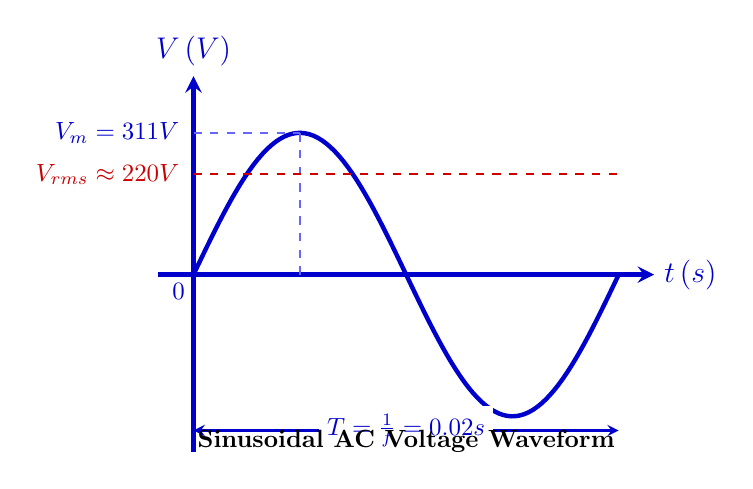
\begin{tikzpicture}[scale=0.9, every node/.style={scale=0.9}]
    % AC Sinusoidal Waveform
    \begin{scope}[shift={(0,0)}]
        % Axes
        \draw[ultra thick, ->, >=stealth, blue!80!black] (-0.5, 0) -- (6.5, 0) node[right, font=\large\bfseries] {$t\,\text{(s)}$};
        \draw[ultra thick, ->, >=stealth, blue!80!black] (0, -2.5) -- (0, 2.8) node[above, font=\large\bfseries] {$V\,\text{(V)}$};

        % Origin
        \node[below left, font=\bfseries, blue!80!black] at (0,0) {$0$};

        % Sinusoidal curve
        \draw[ultra thick, blue!80!black, domain=0:6, samples=100] plot (\x, {2.0*sin(180*\x/3)});

        % Peak Voltage V_m = 311 V
        \draw[dashed, thick, blue!60] (0, 2.0) node[left=2pt, font=\bfseries, blue!80!black] {$V_m = 311\text{ V}$} -- (1.5, 2.0);
        \draw[dashed, thick, blue!60] (1.5, 0) -- (1.5, 2.0);

        % RMS Voltage Line
        \draw[dashed, thick, red!80!black] (0, 1.414) node[left=2pt, font=\bfseries, red!80!black] {$V_{\text{rms}} \approx 220\text{ V}$} -- (6.0, 1.414);

        % Time Period T
        \draw[thick, <->, >=stealth, blue!80!black] (0, -2.2) -- (6.0, -2.2) node[midway, fill=white, font=\bfseries] {$T = \frac{1}{f} = 0.02\text{ s}$};

        \node[below=25pt, font=\bfseries] at (3.0, -1.2) {Sinusoidal AC Voltage Waveform};
    \end{scope}
\end{tikzpicture}  
\end{center}


\begin{choices}
    \choice $200\text{ V},\,50\text{ Hz}$
    \choice $220\text{ V},\,100\text{ Hz}$
    \correctchoice $220\text{ V},\,50\text{ Hz}$
    \choice $200\text{ V},\,100\text{ Hz}$
\end{choices}

\begin{solution}
\subsection*{Understand Standard Sinusoidal AC Equation}
The general equation for a sinusoidal alternating voltage is given by:

$$V = V_m \sin(\omega t)$$

where:
\begin{itemize}
    \item $V_m$ is the peak (maximum) voltage
    \item $\omega = 2\pi f$ is the angular frequency (in rad/s)
    \item $f$ is the frequency (in Hz)
\end{itemize}

\begin{empheq}[box={\mymath[colback=col3!30,drop lifted shadow, rounded corners]}]{equation}\tag{RMS Voltage \& Frequency Formulas}
V_{\text{rms}} = \frac{V_m}{\sqrt{2}}, \quad f = \frac{\omega}{2\pi}
\end{empheq}

\subsection*{Step 1: Determine Peak Voltage and Angular Frequency}
Comparing the given equation $V = 311 \sin 314\,t$ with $V = V_m \sin(\omega t)$:

$$V_m = 311\text{ V}$$

$$\omega = 314\text{ rad/s}$$

\subsection*{Step 2: Calculate RMS Voltage ($V_{\text{rms}}$)}
$$V_{\text{rms}} = \frac{V_m}{\sqrt{2}} = \frac{311}{1.414} \approx 220\text{ V}$$

\subsection*{Step 3: Calculate Frequency ($f$)}
Using $\omega = 2\pi f$:

$$f = \frac{\omega}{2\pi} = \frac{314}{2 \times 3.1416} = \frac{314}{6.2832} \approx 50\text{ Hz}$$

Thus, the RMS voltage is **$220\text{ V}$** and the frequency is **$50\text{ Hz}$**.

Correct Answer: C ($220\text{ V},\,50\text{ Hz}$)
\end{solution}

\clearpage

\section{Physics / Alternating Current}


\subsection{Impedance of a Series LCR Circuit}


In a series $LCR$ circuit, $R = 300\,\Omega$, $L = 0.9\text{ H}$, $C = 2.0\,\mu\text{F}$ and $\omega = 1000\text{ rad/s}$, then impedance of the circuit is \underline{\hspace{2cm}}.

\begin{center}

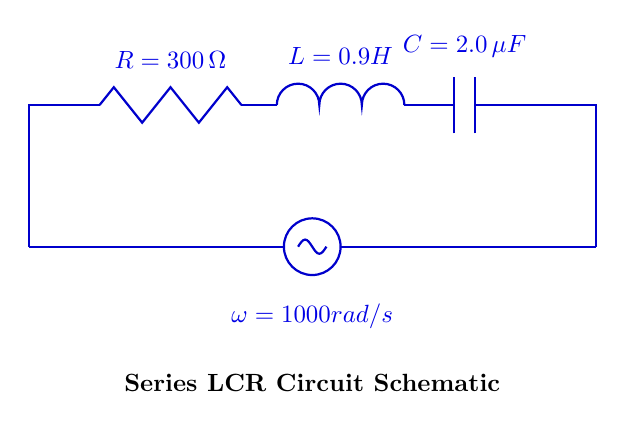
\begin{tikzpicture}[scale=0.9, every node/.style={scale=0.9}]
    % Series LCR Circuit Diagram
    \begin{scope}[shift={(0,0)}]
        % Main Circuit Loop Wires
        \draw[thick, blue!80!black] (-4, 0) -- (-4, 2) -- (-3, 2);
        
        % Resistor (R)
        \draw[thick, blue!80!black] (-3, 2) -- (-2.8, 2.25) -- (-2.4, 1.75) -- (-2.0, 2.25) -- (-1.6, 1.75) -- (-1.2, 2.25) -- (-1.0, 2);
        \node[above=4pt, font=\bfseries, blue!90!black] at (-2.0, 2.25) {$R = 300\,\Omega$};

        \draw[thick, blue!80!black] (-1.0, 2) -- (-0.5, 2);

        % Inductor (L)
        \draw[thick, blue!80!black] (-0.5, 2) arc (180:0:0.3) arc (180:0:0.3) arc (180:0:0.3);
        \node[above=4pt, font=\bfseries, blue!90!black] at (0.4, 2.3) {$L = 0.9\text{ H}$};

        \draw[thick, blue!80!black] (1.3, 2) -- (2.0, 2);

        % Capacitor (C)
        \draw[thick, blue!80!black] (2.0, 1.6) -- (2.0, 2.4);
        \draw[thick, blue!80!black] (2.3, 1.6) -- (2.3, 2.4);
        \node[above=4pt, font=\bfseries, blue!90!black] at (2.15, 2.4) {$C = 2.0\,\mu\text{F}$};

        \draw[thick, blue!80!black] (2.3, 2) -- (4, 2) -- (4, 0);
        \draw[thick, blue!80!black] (-4, 0) -- (-0.4, 0);
        \draw[thick, blue!80!black] (0.4, 0) -- (4, 0);

        % AC Source Symbol
        \draw[thick, fill=white, draw=blue!80!black] (0, 0) circle (0.4);
        \draw[thick, blue!80!black] (-0.2, 0) sin (-0.1, 0.1) cos (0, 0) sin (0.1, -0.1) cos (0.2, 0);
        \node[below=8pt, font=\bfseries, blue!90!black] at (0, -0.4) {$\omega = 1000\text{ rad/s}$};

        \node[below=25pt, font=\bfseries] at (0, -0.8) {Series LCR Circuit Schematic};
    \end{scope}
\end{tikzpicture}  
\end{center}


\begin{choices}
    \choice $900\,\Omega$
    \correctchoice $500\,\Omega$
    \choice $400\,\Omega$
    \choice $1300\,\Omega$
\end{choices}

\begin{solution}
\subsection*{Understand Series LCR Circuit Impedance}
The total opposition to alternating current in a series $LCR$ circuit is defined as the impedance ($Z$). It is calculated using the resistance ($R$), inductive reactance ($X_L$), and capacitive reactance ($X_C$).

\begin{empheq}[box={\mymath[colback=col3!30,drop lifted shadow, rounded corners]}]{equation}\tag{Impedance Formula}
Z = \sqrt{R^2 + (X_L - X_C)^2}
\end{empheq}

\subsection*{Step 1: Calculate Inductive Reactance ($X_L$)}
Using $L = 0.9\text{ H}$ and $\omega = 1000\text{ rad/s}$:

$$X_L = \omega L = 1000 \times 0.9 = 900\,\Omega$$

\subsection*{Step 2: Calculate Capacitive Reactance ($X_C$)}
Using $C = 2.0\,\mu\text{F} = 2.0 \times 10^{-6}\text{ F}$ and $\omega = 1000\text{ rad/s}$:

$$X_C = \frac{1}{\omega C} = \frac{1}{1000 \times 2.0 \times 10^{-6}} = \frac{1}{2 \times 10^{-3}} = 500\,\Omega$$

\subsection*{Step 3: Calculate Net Reactance and Total Impedance ($Z$)}
The difference between the reactances is:

$$|X_L - X_C| = |900\,\Omega - 500\,\Omega| = 400\,\Omega$$

Substitute $R = 300\,\Omega$ and $(X_L - X_C) = 400\,\Omega$ into the impedance formula:

$$Z = \sqrt{(300)^2 + (400)^2} = \sqrt{90000 + 160000} = \sqrt{250000} = 500\,\Omega$$

Thus, the impedance of the circuit is **$500\,\Omega$**.

Correct Answer: B ($500\,\Omega$)
\end{solution}

\clearpage

\begin{comment}
    


\section{Physics / Alternating Current}


\subsection{Resonant Frequency of a Series LC Circuit}


A series resonant AC circuit contains a capacitance $10^{-6}\text{ F}$ and an inductor of $10^{-4}\text{ H}$. The frequency of electrical oscillations will be \underline{\hspace{2cm}}.

\begin{center}

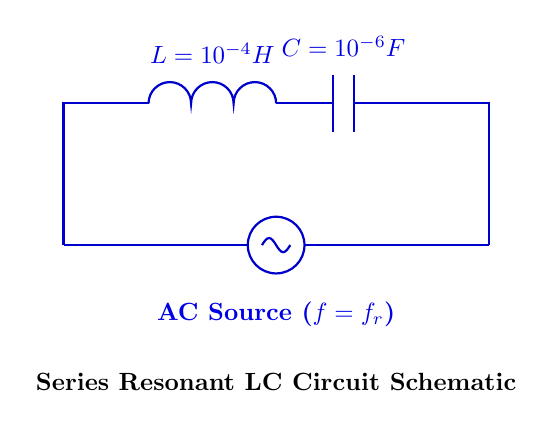
\begin{tikzpicture}[scale=0.9, every node/.style={scale=0.9}]
    % Series Resonant LC Circuit Diagram
    \begin{scope}[shift={(0,0)}]
        % Main Circuit Wires
        \draw[thick, blue!80!black] (-3, 0) -- (-3, 2) -- (-1.8, 2);
        
        % Inductor (L)
        \draw[thick, blue!80!black] (-1.8, 2) arc (180:0:0.3) arc (180:0:0.3) arc (180:0:0.3);
        \node[above=4pt, font=\bfseries, blue!90!black] at (-0.9, 2.3) {$L = 10^{-4}\text{ H}$};

        \draw[thick, blue!80!black] (0.0, 2) -- (0.8, 2);

        % Capacitor (C)
        \draw[thick, blue!80!black] (0.8, 1.6) -- (0.8, 2.4);
        \draw[thick, blue!80!black] (1.1, 1.6) -- (1.1, 2.4);
        \node[above=4pt, font=\bfseries, blue!90!black] at (0.95, 2.4) {$C = 10^{-6}\text{ F}$};

        \draw[thick, blue!80!black] (1.1, 2) -- (3, 2) -- (3, 0);
        \draw[thick, blue!80!black] (-3, 0) -- (-0.4, 0);
        \draw[thick, blue!80!black] (0.4, 0) -- (3, 0);

        % AC Source Symbol
        \draw[thick, fill=white, draw=blue!80!black] (0, 0) circle (0.4);
        \draw[thick, blue!80!black] (-0.2, 0) sin (-0.1, 0.1) cos (0, 0) sin (0.1, -0.1) cos (0.2, 0);
        \node[below=8pt, font=\bfseries, blue!90!black] at (0, -0.4) {AC Source ($f = f_r$)};

        \node[below=25pt, font=\bfseries] at (0, -0.8) {Series Resonant LC Circuit Schematic};
    \end{scope}
\end{tikzpicture}  
\end{center}


\begin{choices}
    \choice $10\text{ Hz}$
    \correctchoice $\frac{10^5}{2\pi}\text{ Hz}$
    \choice $\frac{10}{2\pi}\text{ Hz}$
    \choice $10^5\text{ Hz}$
\end{choices}

\begin{solution}
\subsection*{Understand Resonant Frequency Principle}
At resonance in a series $LC$ or $LCR$ circuit, the inductive reactance $X_L$ equals the capacitive reactance $X_C$, resulting in minimum impedance and maximum current response:

$$X_L = X_C \implies 2\pi f_r L = \frac{1}{2\pi f_r C}$$

\begin{empheq}[box={\mymath[colback=col3!30,drop lifted shadow, rounded corners]}]{equation}\tag{Resonant Frequency Formula}
f_r = \frac{1}{2\pi \sqrt{L C}}
\end{empheq}

\subsection*{Step 1: Substitute Given Values}
Given values:
\begin{itemize}
    \item Inductance, $L = 10^{-4}\text{ H}$
    \item Capacitance, $C = 10^{-6}\text{ F}$
\end{itemize}

Substitute $L$ and $C$ into the resonant frequency equation:

$$\sqrt{L C} = \sqrt{10^{-4} \times 10^{-6}} = \sqrt{10^{-10}} = 10^{-5}\text{ s}$$

\subsection*{Step 2: Calculate Resonant Frequency ($f_r$)}
$$f_r = \frac{1}{2\pi \times 10^{-5}} = \frac{10^5}{2\pi}\text{ Hz}$$

Thus, the frequency of electrical oscillations is **$\frac{10^5}{2\pi}\text{ Hz}$**.

Correct Answer: B ($\frac{10^5}{2\pi}\text{ Hz}$)
\end{solution}

\clearpage


\section{Physics / Alternating Current}


\subsection{Resonant Frequency Calculation of an LC Circuit}


In the given circuit, the resonant frequency is \underline{\hspace{2cm}}.

\begin{center}

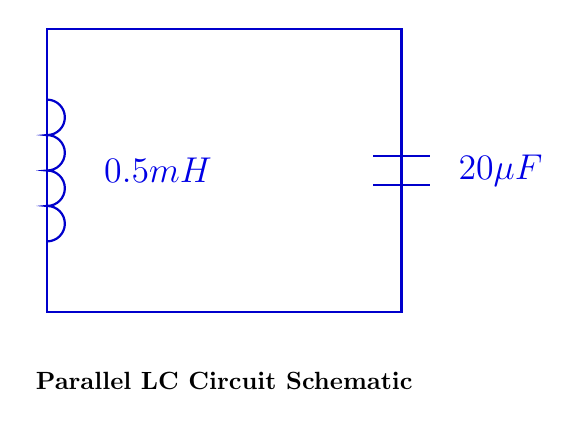
\begin{tikzpicture}[scale=0.9, every node/.style={scale=0.9}]
    % LC Circuit Diagram
    \begin{scope}[shift={(0,0)}]
        % Main Circuit Outer Rectangle / Wires
        \draw[thick, blue!80!black] (-2.5, 0) -- (-2.5, -2) -- (2.5, -2) -- (2.5, 0);
        \draw[thick, blue!80!black] (-2.5, 0) -- (-2.5, 2) -- (2.5, 2) -- (2.5, 0);

        % Inductor (L) on the Left Branch
        \draw[thick, blue!80!black] (-2.5, -1) arc (-90:90:0.25 and 0.25) arc (-90:90:0.25 and 0.25) arc (-90:90:0.25 and 0.25) arc (-90:90:0.25 and 0.25);
        \node[right=8pt, font=\bfseries\Large, blue!90!black] at (-2.1, 0) {$0.5\text{ mH}$};

        % Capacitor (C) on the Right Branch
        \draw[thick, blue!80!black] (2.1, -0.2) -- (2.9, -0.2);
        \draw[thick, blue!80!black] (2.1, 0.2) -- (2.9, 0.2);
        \node[right=8pt, font=\bfseries\Large, blue!90!black] at (2.9, 0) {$20\text{ }\mu\text{F}$};

        \node[below=15pt, font=\bfseries] at (0, -2.2) {Parallel LC Circuit Schematic};
    \end{scope}
\end{tikzpicture}  
\end{center}


\begin{choices}
    \choice $15.92\text{ Hz}$
    \choice $159.2\text{ Hz}$
    \correctchoice $1592\text{ Hz}$
    \choice $15910\text{ Hz}$
\end{choices}

\begin{solution}
\subsection*{Understand Resonant Frequency Principle}
The resonant frequency ($f_r$) of an $LC$ circuit is the natural oscillation frequency at which the inductive reactance ($X_L$) equals the capacitive reactance ($X_C$):

\begin{empheq}[box={\mymath[colback=col3!30,drop lifted shadow, rounded corners]}]{equation}\tag{Resonant Frequency Formula}
f_r = \frac{1}{2\pi \sqrt{L C}}
\end{empheq}

\subsection*{Step 1: Identify Given Parameters}
From the circuit diagram:
\begin{itemize}
    \item Inductance, $L = 0.5\text{ mH} = 0.5 \times 10^{-3}\text{ H}$
    \item Capacitance, $C = 20\text{ }\mu\text{F} = 20 \times 10^{-6}\text{ F}$
\end{itemize}

\subsection*{Step 2: Calculate $L \times C$}
$$L \times C = (0.5 \times 10^{-3}\text{ H}) \times (20 \times 10^{-6}\text{ F}) = 10 \times 10^{-9}\text{ s}^2 = 10^{-8}\text{ s}^2$$

Taking the square root:
$$\sqrt{L C} = \sqrt{10^{-8}} = 10^{-4}\text{ s}$$

\subsection*{Step 3: Calculate Resonant Frequency ($f_r$)}
Substitute into the resonant frequency equation:

$$f_r = \frac{1}{2\pi \times 10^{-4}} = \frac{10^4}{2\pi} = \frac{10000}{2 \times 3.1416} \approx 1591.55\text{ Hz} \approx 1592\text{ Hz}$$

Thus, the resonant frequency of the circuit is **$1592\text{ Hz}$**.

Correct Answer: C ($1592\text{ Hz}$)
\end{solution}

\clearpage


\section{Physics / Electrostatics}


\subsection{Electric Potential and Work Done}


A $200\text{ J}$ of work is done in moving a charge $5\text{ C}$ from a point A where the potential is $-20\text{ V}$ to another point B where potential is $V\text{ volt}$. The value of $V$ at B is \underline{\hspace{2cm}}.

\begin{center}

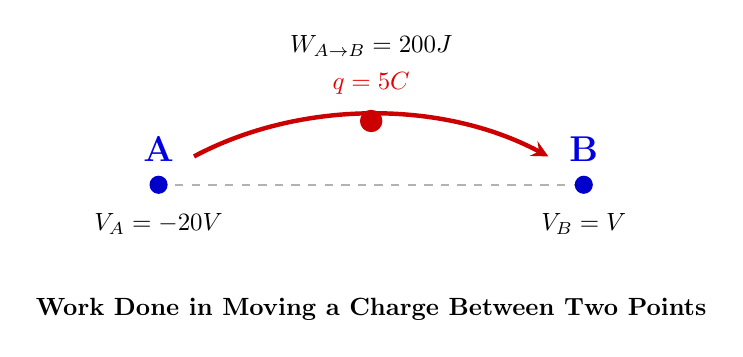
\begin{tikzpicture}[scale=0.9, every node/.style={scale=0.9}]
    % Charge Movement Diagram
    \begin{scope}[shift={(0,0)}]
        % Line connecting Point A and Point B
        \draw[thick, gray!60, dashed] (-3, 0) -- (3, 0);

        % Point A
        \filldraw[blue!80!black] (-3, 0) circle (0.12);
        \node[above=6pt, font=\bfseries\Large, blue!90!black] at (-3, 0) {A};
        \node[below=8pt, font=\bfseries] at (-3, 0) {$V_A = -20\text{ V}$};

        % Point B
        \filldraw[blue!80!black] (3, 0) circle (0.12);
        \node[above=6pt, font=\bfseries\Large, blue!90!black] at (3, 0) {B};
        \node[below=8pt, font=\bfseries] at (3, 0) {$V_B = V$};

        % Moving Charge Arrow and Path
        \draw[ultra thick, ->, >=stealth, red!80!black] (-2.5, 0.4) .. controls (-1, 1.2) and (1, 1.2) .. (2.5, 0.4);
        \filldraw[red!80!black] (0, 0.9) circle (0.15);
        \node[above=3pt, font=\bfseries, red!90!black] at (0, 1.05) {$q = 5\text{ C}$};
        \node[above=18pt, font=\bfseries] at (0, 1.05) {$W_{A \to B} = 200\text{ J}$};

        \node[below=25pt, font=\bfseries] at (0, -0.6) {Work Done in Moving a Charge Between Two Points};
    \end{scope}
\end{tikzpicture}  
\end{center}


\begin{choices}
    \choice $10\text{ V}$
    \correctchoice $20\text{ V}$
    \choice $40\text{ V}$
    \choice $60\text{ V}$
\end{choices}

\begin{solution}
\subsection*{Understand Electric Potential Difference}
The work done ($W_{A \to B}$) by an external agent in moving a charge $q$ from an initial point A to a final point B in an electric field is equal to the product of the charge and the potential difference between the two points:

\begin{empheq}[box={\mymath[colback=col3!30,drop lifted shadow, rounded corners]}]{equation}\tag{Work-Potential Relation}
W_{A \to B} = q (V_B - V_A)
\end{empheq}

\subsection*{Step 1: Identify Given Parameters}
From the problem statement:
\begin{itemize}
    \item Work done, $W_{A \to B} = 200\text{ J}$
    \item Charge moved, $q = 5\text{ C}$
    \item Potential at point A, $V_A = -20\text{ V}$
    \item Potential at point B, $V_B = V$
\end{itemize}

\subsection*{Step 2: Calculate Potential Difference}
Using the formula:

$$200 = 5 \times [V - (-20)]$$

Divide both sides by $5$:

$$40 = V + 20$$

\subsection*{Step 3: Solve for $V$}
$$V = 40 - 20 = 20\text{ V}$$

Thus, the value of the potential $V$ at point B is **$20\text{ V}$**.

Correct Answer: B ($20\text{ V}$)
\end{solution}

\clearpage

\section{Physics / Electromagnetic Induction \& Transient Analysis}


\subsection{Time Constant of an RL Circuit}


The circuit shown in the figure with the switch S open, is in steady state. After the switch S is closed, the time constant of the circuit in seconds is \underline{\hspace{2cm}}.

\begin{center}

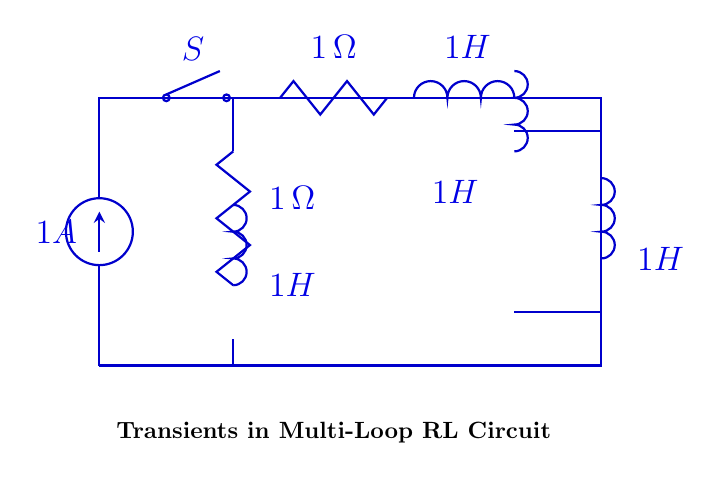
\begin{tikzpicture}[scale=0.85, every node/.style={scale=0.85}]
    % RL Circuit Schematic
    \begin{scope}[shift={(0,0)}]
        % Outer Wire Frame
        \draw[thick, blue!80!black] (-3.5, -2) -- (4, -2) -- (4, 2) -- (-3.5, 2) -- (-3.5, -2);
        
        % Leftmost Branch: Current Source (1 A)
        \draw[thick, fill=white, draw=blue!80!black] (-3.5, 0) circle (0.5);
        \draw[thick, ->, >=stealth, blue!80!black] (-3.5, -0.3) -- (-3.5, 0.3);
        \node[left=6pt, font=\bfseries\Large, blue!90!black] at (-3.5, 0) {$1\text{ A}$};

        % Middle Vertical Branch: 1 Ohm Resistor + 1 H Inductor in Series
        \draw[thick, blue!80!black] (-1.5, 2) -- (-1.5, 1.2);
        % Resistor 1 Ohm
        \draw[thick, blue!80!black] (-1.5, 1.2) -- (-1.75, 1.0) -- (-1.25, 0.6) -- (-1.75, 0.2) -- (-1.25, -0.2) -- (-1.75, -0.6) -- (-1.5, -0.8);
        \node[right=6pt, font=\bfseries\Large, blue!90!black] at (-1.3, 0.5) {$1\,\Omega$};
        % Inductor 1 H
        \draw[thick, blue!80!black] (-1.5, -0.8) arc (-90:90:0.2 and 0.2) arc (-90:90:0.2 and 0.2) arc (-90:90:0.2 and 0.2);
        \node[right=6pt, font=\bfseries\Large, blue!90!black] at (-1.3, -0.8) {$1\text{ H}$};
        \draw[thick, blue!80!black] (-1.5, -2) -- (-1.5, -1.6);

        % Top Horizontal Branch: Switch S + 1 Ohm Resistor + 1 H Inductor
        % Switch S
        \draw[thick, blue!80!black] (-3.5, 2) -- (-2.5, 2);
        \draw[thick, blue!80!black] (-2.5, 2) circle (0.05);
        \draw[thick, blue!80!black] (-1.6, 2) circle (0.05);
        \draw[thick, blue!80!black] (-2.5, 2.05) -- (-1.7, 2.4);
        \node[above=4pt, font=\bfseries\Large, blue!90!black] at (-2.1, 2.3) {$S$};

        \draw[thick, blue!80!black] (-1.55, 2) -- (-0.8, 2);
        % Resistor 1 Ohm
        \draw[thick, blue!80!black] (-0.8, 2) -- (-0.6, 2.25) -- (-0.2, 1.75) -- (0.2, 2.25) -- (0.6, 1.75) -- (0.8, 2);
        \node[above=6pt, font=\bfseries\Large, blue!90!black] at (0, 2.25) {$1\,\Omega$};

        \draw[thick, blue!80!black] (0.8, 2) -- (1.2, 2);
        % Inductor 1 H
        \draw[thick, blue!80!black] (1.2, 2) arc (180:0:0.25) arc (180:0:0.25) arc (180:0:0.25);
        \node[above=6pt, font=\bfseries\Large, blue!90!black] at (2.0, 2.25) {$1\text{ H}$};
        \draw[thick, blue!80!black] (2.7, 2) -- (4, 2);

        % Rightmost Vertical Branch: Two Parallel Inductors (1 H and 1 H)
        % First Inductor (1 H) on Vertical Main Wire
        \draw[thick, blue!80!black] (2.7, 1.2) arc (-90:90:0.2 and 0.2) arc (-90:90:0.2 and 0.2) arc (-90:90:0.2 and 0.2);
        \node[left=6pt, font=\bfseries\Large, blue!90!black] at (2.5, 0.6) {$1\text{ H}$};

        % Second Inductor (1 H) in Parallel Outer Branch
        \draw[thick, blue!80!black] (2.7, 1.5) -- (4.0, 1.5) -- (4.0, 0.8);
        \draw[thick, blue!80!black] (4.0, -0.4) arc (-90:90:0.2 and 0.2) arc (-90:90:0.2 and 0.2) arc (-90:90:0.2 and 0.2);
        \node[right=6pt, font=\bfseries\Large, blue!90!black] at (4.2, -0.4) {$1\text{ H}$};
        \draw[thick, blue!80!black] (4.0, -0.4) -- (4.0, -1.2) -- (2.7, -1.2);

        \node[below=15pt, font=\bfseries] at (0, -2.2) {Transients in Multi-Loop RL Circuit};
    \end{scope}
\end{tikzpicture}  
\end{center}


\begin{choices}
    \correctchoice $1.25$
    \choice $0$
    \choice $1$
    \choice $1.5$
\end{choices}

\begin{solution}
\subsection*{Understand Time Constant Formula for RL Circuits}
The time constant $\tau$ of an $RL$ circuit with respect to its reactive elements is given by:

\begin{empheq}[box={\mymath[colback=col3!30,drop lifted shadow, rounded corners]}]{equation}\tag{RL Time Constant Formula}
\tau = \frac{L_{\text{eq}}}{R_{\text{eq}}}
\end{empheq}

where $L_{\text{eq}}$ and $R_{\text{eq}}$ are the equivalent inductance and equivalent resistance of the circuit connected across the dynamic loop after the switch is closed.

\subsection*{Step 1: Calculate Equivalent Inductance ($L_{\text{eq}}$)}
Looking from the top-right loop when switch $S$ is closed:
\begin{enumerate}
    \item Two inductors of $1\text{ H}$ each on the right vertical branch are connected in parallel:
    $$L_{p} = \frac{1 \times 1}{1 + 1} = 0.5\text{ H}$$
    
    \item This combination is in series with the top inductor of $1\text{ H}$ and the middle branch inductor of $1\text{ H}$:
    $$L_{\text{eq}} = 1\text{ H} + 0.5\text{ H} + 1\text{ H} = 2.5\text{ H}$$
\end{enumerate}

\subsection*{Step 2: Calculate Equivalent Resistance ($R_{\text{eq}}$)}
An ideal current source acts as an **open circuit** for internal resistance calculation:
\begin{itemize}
    \item Removing the $1\text{ A}$ current source leaves the $1\,\Omega$ resistor in the top branch and the $1\,\Omega$ resistor in the middle branch in series connection.
    \item Therefore, total resistance connected across the inductors is:
    $$R_{\text{eq}} = 1\,\Omega + 1\,\Omega = 2\,\Omega$$
\end{itemize}

\subsection*{Step 3: Calculate Time Constant ($\tau$)}
Substitute $L_{\text{eq}} = 2.5\text{ H}$ and $R_{\text{eq}} = 2\,\Omega$ into the time constant formula:

$$\tau = \frac{L_{\text{eq}}}{R_{\text{eq}}} = \frac{2.5}{2} = 1.25\text{ seconds}$$

Thus, the time constant of the circuit after closing switch $S$ is **$1.25$ seconds**.

Correct Answer: A ($1.25$)
\end{solution}

\clearpage


\section{Physics / Electrical Circuits \& Transients}


\subsection{Steady State Analysis of a DC Circuit}


In the circuit shown below, the switch S is closed at $t = 0$. The magnitude of the steady state voltage, in volts, across the $6\,\Omega$ resistor is \underline{\hspace{2cm}}. (round off to two decimal places).

\begin{center}

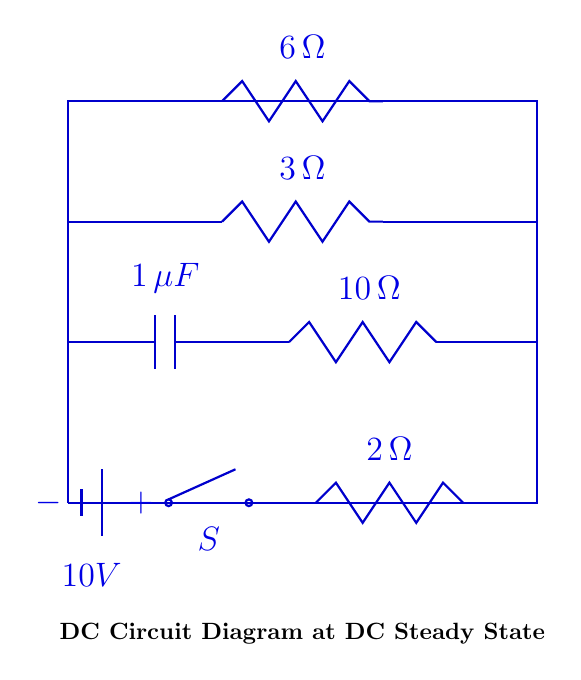
\begin{tikzpicture}[scale=0.85, every node/.style={scale=0.85}]
    % Circuit Schematic
    \begin{scope}[shift={(0,0)}]
        % Main Outer Wire Frame
        \draw[thick, blue!80!black] (-3.5, -3) -- (-3.5, 3) -- (3.5, 3) -- (3.5, -3) -- (-3.5, -3);

        % Top Parallel Branch 1: 6 Ohm Resistor
        \draw[thick, blue!80!black] (-3.5, 3) -- (-1.2, 3);
        \draw[thick, blue!80!black] (-1.2, 3) -- (-0.9, 3.3) -- (-0.5, 2.7) -- (-0.1, 3.3) -- (0.3, 2.7) -- (0.7, 3.3) -- (1.0, 3) -- (1.2, 3);
        \node[above=6pt, font=\bfseries\Large, blue!90!black] at (0, 3.3) {$6\,\Omega$};
        \draw[thick, blue!80!black] (1.2, 3) -- (3.5, 3);

        % Parallel Branch 2: 3 Ohm Resistor
        \draw[thick, blue!80!black] (-3.5, 1.2) -- (-1.2, 1.2);
        \draw[thick, blue!80!black] (-1.2, 1.2) -- (-0.9, 1.5) -- (-0.5, 0.9) -- (-0.1, 1.5) -- (0.3, 0.9) -- (0.7, 1.5) -- (1.0, 1.2) -- (1.2, 1.2);
        \node[above=6pt, font=\bfseries\Large, blue!90!black] at (0, 1.5) {$3\,\Omega$};
        \draw[thick, blue!80!black] (1.2, 1.2) -- (3.5, 1.2);

        % Parallel Branch 3: Capacitor (1 uF) in series with 10 Ohm Resistor
        \draw[thick, blue!80!black] (-3.5, -0.6) -- (-2.2, -0.6);
        % Capacitor 1 uF
        \draw[thick, blue!80!black] (-2.2, -1.0) -- (-2.2, -0.2);
        \draw[thick, blue!80!black] (-1.9, -1.0) -- (-1.9, -0.2);
        \node[above=6pt, font=\bfseries\Large, blue!90!black] at (-2.05, -0.2) {$1\,\mu\text{F}$};
        \draw[thick, blue!80!black] (-1.9, -0.6) -- (-0.2, -0.6);
        % Resistor 10 Ohm
        \draw[thick, blue!80!black] (-0.2, -0.6) -- (0.1, -0.3) -- (0.5, -0.9) -- (0.9, -0.3) -- (1.3, -0.9) -- (1.7, -0.3) -- (2.0, -0.6);
        \node[above=6pt, font=\bfseries\Large, blue!90!black] at (1.0, -0.3) {$10\,\Omega$};
        \draw[thick, blue!80!black] (2.0, -0.6) -- (3.5, -0.6);

        % Bottom Branch: DC Voltage Source (10 V), Switch S, 2 Ohm Resistor
        % Voltage Source (10 V)
        \draw[thick, blue!80!black] (-3.0, -2.5) -- (-3.0, -3.5); % Long plate (+)
        \draw[thick, blue!80!black] (-3.3, -2.8) -- (-3.3, -3.2); % Short plate (-)
        \node[below=8pt, font=\bfseries\Large, blue!90!black] at (-3.15, -3.5) {$10\text{ V}$};
        \node[left=2pt, font=\bfseries\Large, blue!90!black] at (-3.4, -3.0) {$-$};
        \node[right=2pt, font=\bfseries\Large, blue!90!black] at (-2.8, -3.0) {$+$};

        % Switch S
        \draw[thick, blue!80!black] (-2.0, -3) circle (0.05);
        \draw[thick, blue!80!black] (-0.8, -3) circle (0.05);
        \draw[thick, blue!80!black] (-2.0, -2.95) -- (-1.0, -2.5);
        \node[below=4pt, font=\bfseries\Large, blue!90!black] at (-1.4, -3.1) {$S$};

        % Resistor 2 Ohm
        \draw[thick, blue!80!black] (-0.75, -3) -- (0.2, -3);
        \draw[thick, blue!80!black] (0.2, -3) -- (0.5, -2.7) -- (0.9, -3.3) -- (1.3, -2.7) -- (1.7, -3.3) -- (2.1, -2.7) -- (2.4, -3);
        \node[above=6pt, font=\bfseries\Large, blue!90!black] at (1.3, -2.7) {$2\,\Omega$};
        \draw[thick, blue!80!black] (2.4, -3) -- (3.5, -3);

        \node[below=25pt, font=\bfseries] at (0, -3.8) {DC Circuit Diagram at DC Steady State};
    \end{scope}
\end{tikzpicture}  
\end{center}


\begin{solution}
\subsection*{Understand DC Steady State Behavior}
In a DC circuit operating under steady state condition ($t \to \infty$):
\begin{itemize}
    \item A capacitor behaves as an **open circuit** because its capacitive reactance $X_C = \frac{1}{2\pi f C} \to \infty$ for DC ($f = 0\text{ Hz}$).
    \item Consequently, no current flows through the branch containing the $1\,\mu\text{F}$ capacitor and $10\,\Omega$ resistor.
\end{itemize}

\begin{empheq}[box={\mymath[colback=col3!30,drop lifted shadow, rounded corners]}]{equation}\tag{Parallel Resistance Formula}
R_{p} = \frac{R_1 \times R_2}{R_1 + R_2}
\end{empheq}

\subsection*{Step 1: Simplify the Parallel Combination}
The $6\,\Omega$ and $3\,\Omega$ resistors are connected in parallel. Their equivalent resistance $R_p$ is:

$$R_p = \frac{6 \times 3}{6 + 3} = \frac{18}{9} = 2\,\Omega$$

\subsection*{Step 2: Calculate Total Circuit Resistance ($R_{\text{total}}$)}
Since the capacitor branch is open, the current flows only through $R_p$ and the series $2\,\Omega$ resistor in the bottom branch:

$$R_{\text{total}} = R_p + 2\,\Omega = 2\,\Omega + 2\,\Omega = 4\,\Omega$$

\subsection*{Step 3: Calculate Main Source Current ($I$)}
Using Ohm's Law for the total circuit with supply voltage $V_s = 10\text{ V}$:

$$I = \frac{V_s}{R_{\text{total}}} = \frac{10\text{ V}}{4\,\Omega} = 2.5\text{ A}$$

\subsection*{Step 4: Calculate Steady State Voltage Across $6\,\Omega$ Resistor}
Since the $6\,\Omega$ and $3\,\Omega$ resistors are in parallel, the voltage across the $6\,\Omega$ resistor is equal to the voltage drop across their equivalent resistance $R_p$:

$$V_{6\,\Omega} = V_{R_p} = I \times R_p = 2.5\text{ A} \times 2\,\Omega = 5.00\text{ V}$$

Thus, the magnitude of the steady state voltage across the $6\,\Omega$ resistor is **$5$** (or **$5.00\text{ V}$**).

Final Answer: $5$ or $5.00$
\end{solution}

\clearpage

\end{comment}